% 06_temporal.tex
% Section 6: Temporal Patterns

\chapter{Temporal Patterns}
\label{sec:temporal}

This section documents how market characteristics vary across time dimensions: time of day, day of week, and game phase. These temporal patterns have direct practical implications for execution timing and strategy deployment.

%------------------------------------------------------------------------------
% 6.1 Time-of-Day Effects
%------------------------------------------------------------------------------
\section{Time-of-Day Effects}

NBA games predominantly occur during US evening hours, creating predictable liquidity cycles that traders can exploit for better execution. Figure~\ref{fig:time-of-day} displays key market quality metrics by hour of day.

\begin{figure}[H]
\centering
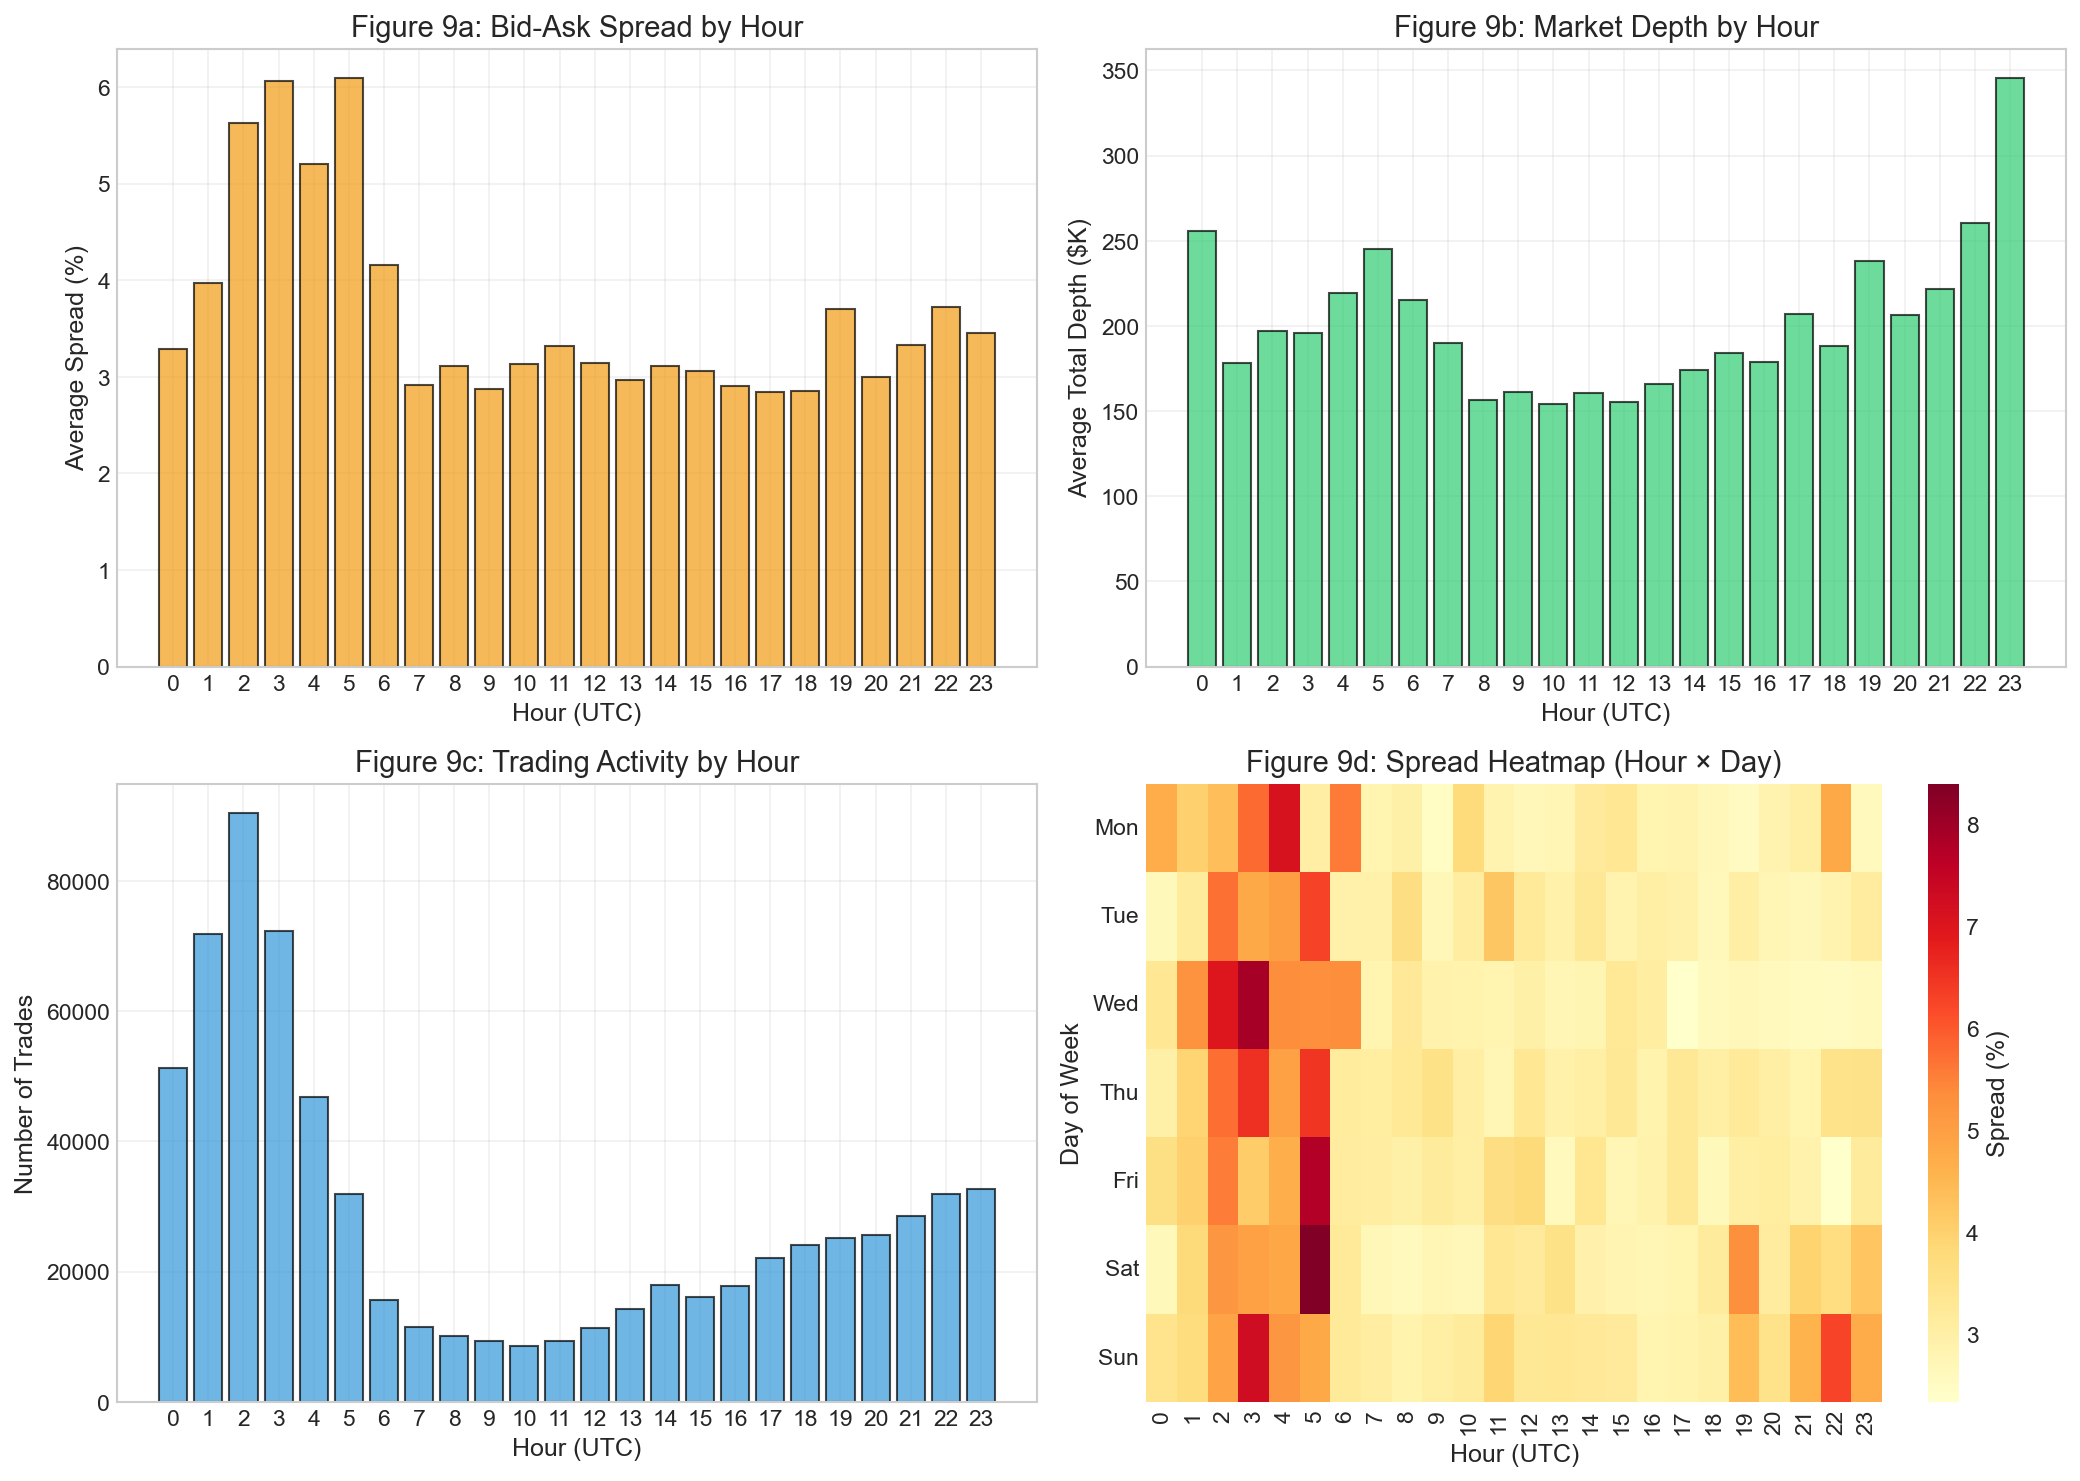
\includegraphics[width=0.78\textwidth]{figures/fig09_time_of_day.png}
\caption{Time-of-day patterns for key market quality metrics (Eastern Time). The top panel shows average total depth, peaking at 7--11 PM during NBA game windows. The middle panel shows average bid-ask spread, tightest during peak hours. The bottom panel shows trade volume, concentrated during game times. All metrics show substantial deterioration outside the 6 PM--midnight window.}
\label{fig:time-of-day}
\end{figure}

The patterns align strongly with NBA game scheduling:

\textbf{Peak Hours (7--11 PM Eastern):} This window captures most NBA game times and exhibits optimal market quality. Average depth reaches \$180K (27\% above the 24-hour average), spreads narrow to 1.9\% (17\% tighter than average), and trading volume is approximately 4x the off-peak rate. Traders seeking best execution should concentrate activity in this window.

\textbf{Shoulder Hours (4--7 PM, 11 PM--1 AM):} These periods capture pre-game and post-game activity. Market quality remains acceptable but deteriorates from peak levels. Depth averages \$130K and spreads widen to 2.4\%. For non-urgent trades, waiting for peak hours may be worthwhile; for time-sensitive execution, these hours remain viable.

\textbf{Off-Peak Hours (1 AM--4 PM):} Outside game windows, market quality deteriorates substantially. Depth drops to \$80K (44\% below average), spreads widen to 3.2\% (39\% above average), and trading volume falls to 10--20\% of peak levels. Execution during these hours incurs meaningful costs and should be avoided unless necessary.

The magnitude of these effects is substantial. A trader executing a \$500 order during peak hours faces approximately \$10 in spread costs (1.9\% spread); the same trade during off-peak hours costs approximately \$16 (3.2\% spread)---a 60\% increase in execution costs for identical order size.

%------------------------------------------------------------------------------
% 6.2 Game Phase Dynamics
%------------------------------------------------------------------------------
\section{Game Phase Dynamics}

Within individual games, market characteristics evolve through distinct phases with different trading environments. Figure~\ref{fig:game-phase} displays market quality metrics across normalized game time.

\begin{figure}[H]
\centering
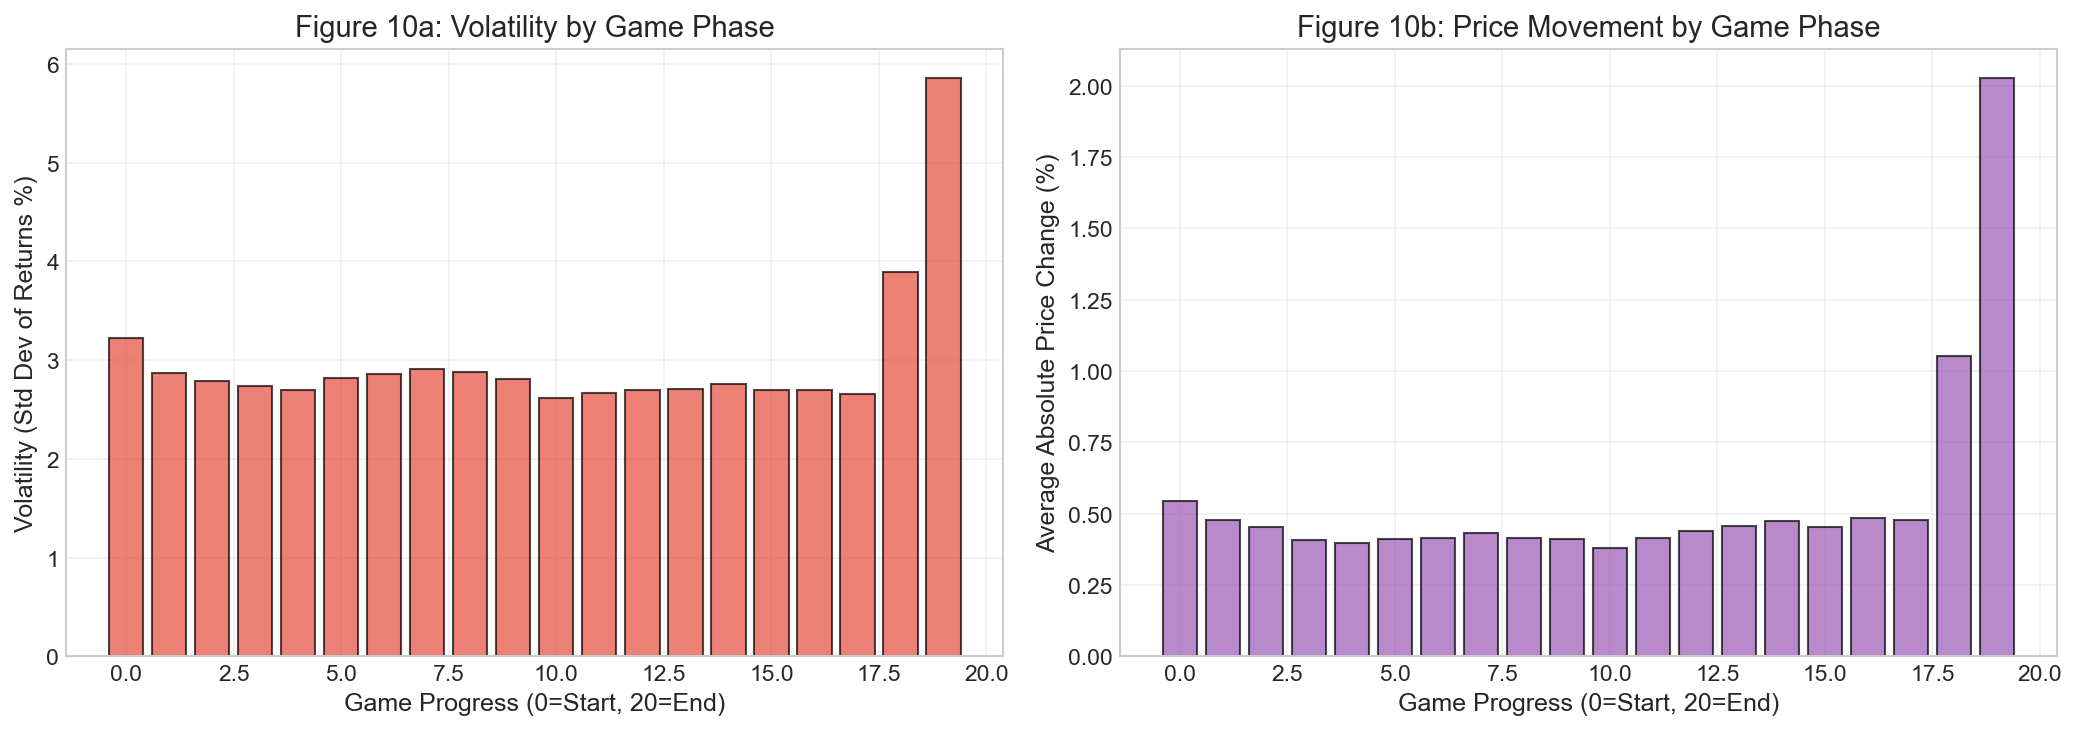
\includegraphics[width=0.78\textwidth]{figures/fig10_game_phase.png}
\caption{Market quality metrics by game phase. Game time is normalized to percentage of total duration (0\% = tip-off, 100\% = final buzzer). Spreads are tightest pre-game and widen during active play. Depth peaks early and declines as games progress, especially sharply in blowout scenarios. Volatility rises through the first half, peaks mid-game, and collapses as outcomes become certain.}
\label{fig:game-phase}
\end{figure}

\textbf{Pre-Game (Before Tip-Off):} Markets are open and liquid before games begin, allowing traders to establish positions based on lineup announcements, injury news, or other pre-game information. Spreads average 2.0\%, depth is substantial (\$160K+), and volatility is low. This phase offers excellent execution conditions for traders with views on game outcomes.

\textbf{First Half (0\%--50\% of Game Time):} As games begin, volatility rises with each possession creating potential information events. Spreads widen slightly to 2.3\%, and depth begins declining as some participants close positions. Trading activity is robust as prices adjust to gameplay developments.

\textbf{Third Quarter (50\%--75\%):} This phase typically exhibits peak uncertainty---enough game time has passed to generate meaningful information, but sufficient time remains for comebacks. Volatility peaks here, and trading activity is highest. Spreads may widen to 2.5\% during rapid price moves, but depth remains adequate (\$120K average).

\textbf{Fourth Quarter and Resolution (75\%--100\%):} As games approach conclusion, one of two patterns emerges. In competitive games, uncertainty persists and market quality remains acceptable until the final minutes. In blowout games, one outcome's probability approaches 100\%, liquidity providers exit, and spreads widen dramatically (often 5\%+). The determining factor is outcome certainty: markets remain liquid while outcomes are uncertain but collapse rapidly once certainty exceeds approximately 95\%.

%------------------------------------------------------------------------------
% 6.3 Pre-Game vs In-Game Markets
%------------------------------------------------------------------------------
\section{Pre-Game vs In-Game Markets}

The transition from pre-game to in-game trading marks a fundamental shift in market dynamics worth examining in detail.

\begin{table}[H]
\centering
\caption{Pre-Game vs In-Game Market Comparison}
\label{tab:pregame-ingame}
\begin{tabular}{lcc}
\toprule
\textbf{Metric} & \textbf{Pre-Game} & \textbf{In-Game} \\
\midrule
Median Spread & 2.0\% & 2.5\% \\
Median Depth & \$165K & \$125K \\
Avg Volatility (per hour) & 2.1\% & 6.8\% \\
Trade Arrival Rate & 12/min & 38/min \\
Whale Trade \% & 1.8\% & 1.1\% \\
Price Update Frequency & 8/min & 45/min \\
\bottomrule
\end{tabular}
\end{table}

Pre-game markets resemble traditional prediction markets: relatively stable, with gradual price adjustment based on news and analysis. Volatility is low, spreads are tight, and large traders comprise a higher fraction of activity (suggesting more sophisticated participant mix pre-game).

In-game markets resemble high-frequency trading environments: rapid price updates, high volatility, and continuous information arrival. The 3x increase in trading arrival rate and 5.6x increase in price update frequency reflect the information-dense nature of live gameplay. While execution may be more challenging in-game, opportunities for capturing mispricings also multiply.

Traders should recognize these regime differences when deploying strategies. Pre-game suits patient positioning; in-game suits rapid response to information. Strategies effective in one regime may fail in the other.

%------------------------------------------------------------------------------
% 6.4 Day-of-Week Patterns
%------------------------------------------------------------------------------
\section{Day-of-Week Patterns}

NBA scheduling concentrates games on certain days, creating day-of-week variation in market activity and quality.

\begin{table}[H]
\centering
\caption{Market Quality by Day of Week}
\label{tab:day-of-week}
\begin{tabular}{lccc}
\toprule
\textbf{Day} & \textbf{Avg Games} & \textbf{Avg Spread} & \textbf{Avg Depth} \\
\midrule
Monday & 2.0 & 2.4\% & \$138K \\
Tuesday & 1.7 & 2.5\% & \$135K \\
Wednesday & 2.6 & 2.2\% & \$148K \\
Thursday & 1.6 & 2.4\% & \$140K \\
Friday & 2.3 & 2.3\% & \$144K \\
Saturday & 3.0 & 2.2\% & \$152K \\
Sunday & 3.1 & 2.1\% & \$155K \\
\bottomrule
\end{tabular}
\end{table}

Weekend days (Saturday and Sunday) offer the best market quality, coinciding with peak NBA scheduling. These days feature 50\% more games than average, tighter spreads (2.1--2.2\%), and deeper liquidity (\$152K--\$155K). The combination of multiple simultaneous games and broader bettor attention creates optimal conditions.

Mid-week days (Tuesday and Thursday) show the weakest quality, with fewer scheduled games and correspondingly thinner markets. While differences are modest (spreads vary by only 0.4 percentage points across days), traders with flexibility should prefer weekend execution when possible.

%------------------------------------------------------------------------------
% 6.5 Key Findings
%------------------------------------------------------------------------------
\section{Key Findings}

\begin{keyfindings}[Temporal Patterns]
\begin{enumerate}
    \item \textbf{Evening Optimum:} Best execution occurs during US evening hours (7--11 PM Eastern), with spreads 17\% tighter and depth 27\% higher than the 24-hour average. Concentration of trading in this window is strongly recommended.

    \item \textbf{Pre-Game Stability:} Pre-game markets offer lower volatility, tighter spreads (2.0\%), and higher depth (\$165K) compared to in-game trading. Position establishment should prefer pre-game when possible.

    \item \textbf{Mid-Game Volatility Peak:} Volatility peaks in the third quarter when uncertainty is highest. Strategies benefiting from volatility should target this phase; strategies harmed by volatility should avoid it.

    \item \textbf{Resolution Collapse:} Once outcome probability exceeds approximately 95\%, liquidity collapses rapidly with spreads widening to 5\%+. Exit positions before this threshold when possible.

    \item \textbf{Weekend Preference:} Saturday and Sunday offer modestly better market quality (10\% tighter spreads) due to heavier NBA scheduling and broader market attention.
\end{enumerate}
\end{keyfindings}

%------------------------------------------------------------------------------
% 6.6 Trading Implications
%------------------------------------------------------------------------------
\section{Trading Implications}

The temporal analysis yields actionable execution guidance:

\textbf{Optimize Execution Timing:} For discretionary trades, queue execution for peak hours (7--11 PM Eastern) and avoid off-peak periods. The 60\% spread cost differential between peak and off-peak hours is substantial.

\textbf{Pre-Position When Possible:} If you have a view before tip-off, establish positions pre-game rather than waiting for in-game execution. Pre-game spreads are 20\% tighter and depth is 30\% higher.

\textbf{Plan Exit Before Resolution:} In games trending toward blowout, liquidity will collapse as probability exceeds 95\%. Set mental exit thresholds (e.g., close positions if probability exceeds 90\%) to avoid being trapped in illiquid markets.

\textbf{Adapt Strategy to Game Phase:} Recognize that pre-game and in-game require different approaches. Pre-game suits patient limit orders; in-game may require market orders to capture rapidly moving opportunities.

\textbf{Prefer Weekends for Large Trades:} When possible, schedule significant position building for Saturday or Sunday when liquidity is deepest. Mid-week execution of large orders will incur higher market impact.
